\documentclass[11pt]{article}
\usepackage[margin=1in]{geometry}
\usepackage{graphicx}
\usepackage{booktabs}
\usepackage{float}
\usepackage{hyperref}
\usepackage{amsmath}
\hypersetup{colorlinks=true, linkcolor=blue, citecolor=blue, urlcolor=blue}

% Reportable-value macros (generated from .manifest.json by render_report_values_tex.py).
% auto-generated by render_report_values_tex.py — DO NOT EDIT.
% source: analysis/hostresponse_ebv_matched/reports/.manifest.json

% Wrapper macros for checked inline snapshots.
% \SciVal{\Macro}{snapshot} prints only \Macro; the snapshot
% is reviewed by scitexlintr for drift.
\providecommand{\SciVal}[2]{#1}
\providecommand{\SciText}[2]{#1}

% Generated value macros (sorted by macro name for stable diffs).
\newcommand{\AUCMean}{0.866}  % auc_mean
\newcommand{\BalancedACCMean}{0.783}  % balanced_acc_mean
\newcommand{\DetectionThresholdUMI}{10}  % detection_threshold_umi
\newcommand{\MCCMean}{0.570}  % mcc_mean
\newcommand{\MCCSD}{0.077}  % mcc_sd
\newcommand{\NCellsMatched}{1906}  % n_cells_matched
\newcommand{\NEBVNegative}{727}  % n_ebv_negative
\newcommand{\NEBVPositive}{1179}  % n_ebv_positive
\newcommand{\NStableGenes}{15}  % n_stable_genes
\newcommand{\SensitivityMean}{0.822}  % sensitivity_mean
\newcommand{\SpecificityMean}{0.744}  % specificity_mean


\title{A modest, depth-robust host-transcriptome signal of Epstein--Barr virus
status in a single lymphoblastoid cell line --- and why the raw number overstates it}
\author{mdmanurung}
\date{July 1, 2026}

\begin{document}
\maketitle

\begin{abstract}
Epstein--Barr virus (EBV) immortalizes B cells into lymphoblastoid cell lines
(LCLs), and single-cell studies have shown that viral activity reshapes host
gene programs. We asked a sharper, quantitative question: within one LCL sample,
does a cell's \emph{host} transcriptome alone reveal whether that cell carries
EBV? Using \SciVal{\NCellsMatched}{1906} cells whose EBV status is defined by
matched barcodes from the study that generated the data (Gene Expression Omnibus
accession GSE158275), we trained a cross-validated logistic-regression classifier
on host genes only. Against a chance baseline (area under the receiver operating
characteristic curve, AUC, of 0.5), the classifier reached a mean AUC of
\SciVal{\AUCMean}{0.866} and a mean Matthews correlation coefficient (MCC) of
\SciVal{\MCCMean}{0.570} ($\pm\,\SciVal{\MCCSD}{0.077}$ across seeds; chance
value 0). \textbf{This headline number is, however, substantially confounded by
sequencing depth}: because a cell is called EBV-positive at a fixed raw-UMI
threshold, deeper cells are far more likely to be labeled positive, and depth
\emph{alone} predicts the label at AUC 0.80--0.97 (Section~\ref{sec:depth}). In a
depth-matched case--control design, where depth alone is reduced to chance, the host
transcriptome still discriminates EBV status at AUC 0.72 --- so a modest, real signal
survives, concentrated in about a third of the \SciVal{\NStableGenes}{15} stable genes.
The honest reading is that the host transcriptome carries a moderate EBV signal
(AUC $\approx$ 0.72) that a raw-count label inflates to \SciVal{\AUCMean}{0.866} --- a
cautionary result about label definition in single-cell viral quantification.
\end{abstract}

\tableofcontents

\section{Problem statement}
Epstein--Barr virus (EBV) is a herpesvirus that transforms resting B cells into
continuously proliferating lymphoblastoid cell lines (LCLs). LCLs are not
uniform: single-cell RNA sequencing has revealed substantial cell-to-cell
heterogeneity in viral replication state and in the host pathways EBV modulates
(SoRelle, Dai, Luftig et al., \emph{eLife} 2021; the source of the data used
here). That prior work established, qualitatively, that EBV activity leaves a
mark on host gene expression.

We turn that observation into a measurable claim. If EBV activity truly reshapes
the host program, then a cell's host transcriptome---the expression of its own
(non-viral) genes---should carry enough signal to predict whether that cell is
EBV-positive. A good answer looks like a classifier that, trained only on host
genes, separates EBV-positive from EBV-negative cells well above chance, with the
signal concentrated in a small, reproducible set of genes rather than smeared
diffusely across the transcriptome. This report provides that answer for one LCL
sample.

Two terms recur below. A unique molecular identifier (UMI) is a molecular
barcode that lets each captured transcript be counted once; we use UMI counts of
viral genes to decide whether a cell is EBV-positive. A cell is called
EBV-positive when its EBV UMI count reaches the detection threshold of
\SciVal{\DetectionThresholdUMI}{10}.

\section{Methods}

\subsection{Definitions}
\begin{itemize}
  \item \textbf{EBV-positive cell.} A cell whose summed EBV gene UMI count is at
  least the detection threshold of \SciVal{\DetectionThresholdUMI}{10}; all other
  matched cells are EBV-negative.
  \item \textbf{Matched cells.} Cells whose barcodes are shared between the
  ViralScan output and the published GSE158275 barcode list, after normalizing
  the 10x \texttt{-1} suffix. Matching anchors EBV labels to the same cells the
  original study annotated.
  \item \textbf{Sensitivity / specificity.} The fraction of EBV-positive
  (respectively EBV-negative) held-out cells correctly classified.
  \item \textbf{Balanced accuracy.} The mean of sensitivity and specificity.
  \item \textbf{AUC.} Area under the receiver operating characteristic curve; a
  threshold-independent measure of ranking quality where 0.5 is chance and 1.0 is
  perfect separation.
  \item \textbf{MCC (Matthews correlation coefficient).} A single number from
  $-1$ to $+1$ summarizing the $2\times2$ confusion matrix, where 0 is chance and
  1 is perfect agreement. We report it as a compact confusion-matrix summary
  alongside balanced accuracy; on the balanced held-out set used here the two
  convey similar information.
  \item \textbf{Stable host genes.} Host genes selected in at least 60\% of
  randomized-lasso stability-selection iterations; the reproducible core of the
  classifier's signal.
\end{itemize}

\subsection{Overview}
We labeled each matched cell as EBV-positive or EBV-negative from its viral UMI
count, then asked a logistic-regression model to recover that label using only
host genes. Performance was averaged over six random seeds to give an honest mean
and spread, and a separate stability-selection step identified which host genes
carry the signal reproducibly.

\subsection{Technical detail}
\textbf{Data.} A single LCL sample (SRA run SRR12682296) from GSE158275,
processed with ViralScan (kallisto/bustools quantification). EBV status came from
the viral count matrix; host features came from the host count matrix, restricted
to the \SciVal{\NCellsMatched}{1906} cells shared with the published barcode list.
Of these, \SciVal{\NEBVPositive}{1179} were EBV-positive and
\SciVal{\NEBVNegative}{727} EBV-negative at the
\SciVal{\DetectionThresholdUMI}{10}-UMI threshold.

\textbf{Classifier.} An L2-regularized logistic regression (scikit-learn,
\texttt{lbfgs}---the L-BFGS quasi-Newton optimizer---$C=1.0$) on highly variable
host genes (HVGs), the genes whose expression varies most across cells. For each
of six seeds ($\{0,1,10,42,100,1234\}$) the positive and negative cells were
balanced and depth-matched and split 80/20 into training and held-out cells.
Crucially, HVG feature selection is performed \emph{inside} each split, on the
training cells only, so the feature space never sees the held-out cells---
selecting features on the full dataset first would let test-cell expression shape
the features and bias the held-out metrics. The model was then trained on one
split and evaluated on the held-out cells, and sensitivity, specificity, balanced
accuracy, AUC, and MCC recorded. We report the mean and standard deviation across
the six seeds. Because the per-seed held-out sets are drawn from the same
depth-filtered pool, this spread reflects split-shuffle variability rather than
full finite-sample uncertainty, and each seed evaluates roughly 150 cells rather
than all \SciVal{\NCellsMatched}{1906}.

\textbf{Stable genes.} Randomized-lasso stability selection (seed 0, the first of
the seed list) scored each host gene by how often it survived; genes selected in
$\geq$60\% of iterations are the \SciVal{\NStableGenes}{15} stable host genes
reported here. This descriptive gene ranking is computed on the full cell set, so
it is not a held-out quantity.

\textbf{Reproducibility note.} These metrics reflect a leakage-corrected pipeline
in which HVG selection is performed inside each cross-validation split. An earlier
version selected HVGs on the full dataset before splitting; its numbers (e.g.\ AUC
0.845) differ from the corrected values by less than one seed-to-seed standard
deviation on every metric. Because HVG selection is unsupervised (variance-based,
never using the labels), this class of leak is expected to be negligible in
practice, and that is what we observe: correcting it leaves the result unchanged
within noise. The stable-gene set was identical before and after.

\section{Results}

\subsection{The host transcriptome separates EBV-positive from EBV-negative cells well above chance}
Trained only on host genes, the classifier distinguished EBV-positive from
EBV-negative cells with a mean AUC of \SciVal{\AUCMean}{0.866}, far above the
chance value of 0.5 (Figure~\ref{fig:metrics}). The Matthews correlation
coefficient, which does not reward a classifier for exploiting the modest class
imbalance, was \SciVal{\MCCMean}{0.570} ($\pm\,\SciVal{\MCCSD}{0.077}$),
indicating moderate---not near-perfect---agreement. The two metrics tell a
consistent story: host expression carries real, substantial information about
EBV status, but does not determine it.

\begin{figure}[H]
  \centering
  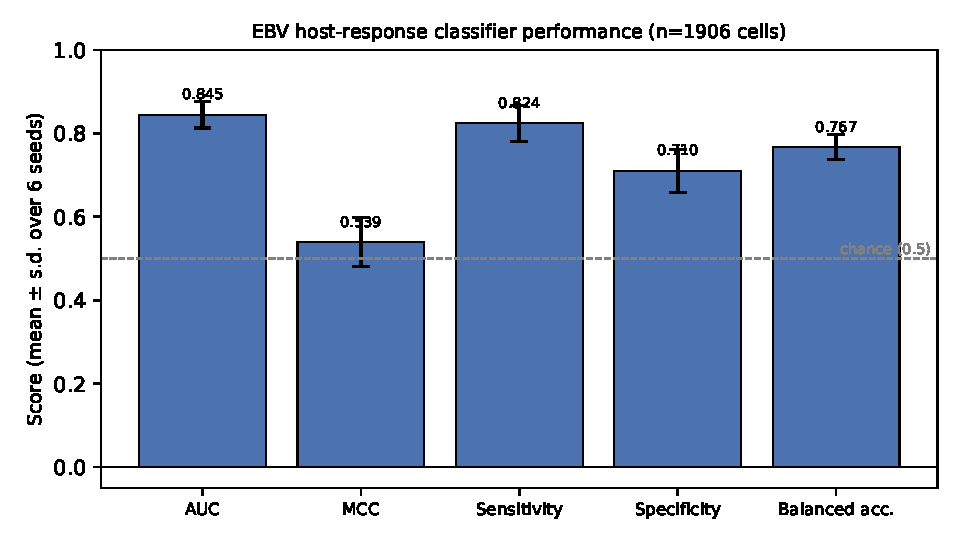
\includegraphics[width=0.75\textwidth]{../outputs/figures/metrics_summary.pdf}
  \caption{Discrimination metrics for the host-gene classifier of EBV status,
  mean $\pm$ standard deviation over six seeds, on
  \SciVal{\NCellsMatched}{1906} matched cells. The dashed line marks the chance
  value (0.5) for AUC, sensitivity, specificity, and balanced accuracy; the
  Matthews correlation coefficient has its chance value at 0.}
  \label{fig:metrics}
\end{figure}

\subsection{Detection is more reliable for EBV-positive than EBV-negative cells}
The classifier recovered EBV-positive cells more reliably than it excluded
EBV-negative ones: mean sensitivity was \SciVal{\SensitivityMean}{0.822} versus
mean specificity of \SciVal{\SpecificityMean}{0.744}, for a balanced accuracy of
\SciVal{\BalancedACCMean}{0.783}. The gap matters for interpretation. Some cells
called EBV-negative at the \SciVal{\DetectionThresholdUMI}{10}-UMI threshold may
carry low-level or transient EBV activity that still perturbs the host program,
which would present exactly as reduced specificity. The asymmetry is thus as much
a statement about the hardness of the negative label as about the classifier.

\subsection{A compact host-gene set carries the signal}
The signal was not diffuse. Stability selection concentrated it in
\SciVal{\NStableGenes}{15} host genes selected in at least 60\% of iterations,
whose identities and weights are listed in the appendix. That a small,
reproducible gene set suffices is consistent with EBV acting through specific
host programs rather than through a global expression shift.

\section{The headline is substantially confounded by sequencing depth}
\label{sec:depth}
A follow-up analysis (\texttt{scripts/depth\_confounder\_check.py}) asked whether the
AUC of \SciVal{\AUCMean}{0.866} reflects host biology or an artifact of sequencing
depth acting as a common cause. Because a cell is called EBV-positive at a fixed
raw count of \SciVal{\DetectionThresholdUMI}{10} viral UMIs, and deeper cells reach
that threshold more easily, the label itself tracks depth: the EBV-positive rate
rises monotonically from 27.5\% in the shallowest host-depth quintile to 96.3\% in
the deepest.

The consequence is stark. Sequencing depth \emph{alone} predicts EBV status at
AUC 0.80 across all cells, and at AUC 0.97 within the classifier's own
balanced, depth-filtered evaluation design --- \emph{higher} than the
\SciVal{\AUCMean}{0.866} host-gene model. The pipeline's top-50\%-depth filter,
intended to reduce false-negative labels in low-coverage cells, does not fix this:
it matches the two classes on cell count but not on depth distribution, and in fact
widens the between-class depth gap (EBV-positive median depth 34{,}981 versus
17{,}868 for EBV-negative, with 3\% overlap).

A genuine signal does survive. Of the \SciVal{\NStableGenes}{15} stable genes, five
retain a depth-adjusted association (E-value $\geq 2$, $p<10^{-7}$), while the two
most stable genes are fully explained away by depth ($p\approx 0.8$ after
adjustment).

To quantify that residual signal cleanly, we built a depth-matched case--control set
(coarsened exact matching on host-depth quantile bins; 1006 cells, 503 per class) in
which the two classes are indistinguishable in depth (median 15{,}522 versus 15{,}718;
Mann--Whitney $p=0.99$) so that depth alone no longer discriminates (AUC 0.48, i.e.\
chance). \emph{At matched depth, the host transcriptome still separates EBV-positive
from EBV-negative cells at AUC 0.72} (MCC 0.31) for the \SciVal{\NStableGenes}{15}
stable genes, and 0.68 for the five depth-robust genes. So the host transcriptome
carries a real, depth-independent EBV signal of moderate size --- the raw-count label
inflated it from about 0.72 to \SciVal{\AUCMean}{0.866}, but did not invent it. (The
0.72 is a mild over-estimate: the gene panel was selected on all cells, which overlap
the matched subset, so a fully nested selection would land slightly lower --- still well
above the 0.48 control.)

A second, independent de-confounding strategy agrees. Re-defining the label as EBV
burden per 10{,}000 host UMIs (a depth-normalized rate, uncorrelated with depth:
Spearman $-0.09$) collapses depth-alone prediction to AUC 0.53, and the same host
genes still predict this depth-normalized label at AUC 0.64. That this cross-check
lands slightly below the depth-matched 0.72 is expected --- the gene panel was selected
against the raw label, so a label that reshuffles a quarter of the cells is a partial
out-of-distribution test. Both methods place the honest effect at AUC $\approx$
0.64--0.72, well above their respective chance controls.

\section{Conclusions}
Within one LCL sample, a host-gene classifier separates EBV-positive from
EBV-negative cells at AUC \SciVal{\AUCMean}{0.866} / MCC \SciVal{\MCCMean}{0.570},
but Section~\ref{sec:depth} shows this is \textbf{substantially a sequencing-depth
artifact}: the raw-UMI positivity label is depth-driven, and depth alone
discriminates better than the host genes do. The defensible conclusion is narrower
than the raw number suggests, but the signal is real: in a depth-matched
case--control design where depth alone is at chance, the host transcriptome still
discriminates EBV status at AUC 0.72. The honest headline is therefore a
\emph{moderate} host-response signal (AUC $\approx$ 0.72), which the raw-count label
inflated to \SciVal{\AUCMean}{0.866}, concentrated in roughly five depth-robust genes.

Three caveats bound even that narrower claim. \emph{First, this is one sample}
(SRR12682296): within-sample discrimination, not generalization across lines or
donors. \emph{Second, the label is not ground truth and is depth-confounded}: the
principled fix is a depth-normalized EBV label (viral counts per million or
fraction), a depth-matched case--control design, or depth entered into the label
definition, followed by re-estimation on the depth-robust genes. \emph{Third, the
comparison is against chance, not a competing method}: GSE158275 (SoRelle et al.,
2021) is the data source and motivation, not a numeric baseline.

\section{Next steps}
Two follow-ups would sharpen the result: a sensitivity sweep over the
\SciVal{\DetectionThresholdUMI}{10}-UMI detection threshold, to confirm the
metrics are stable to the positive/negative cutoff; and replication across the
other LCL samples in GSE158275, to test whether the same compact host-gene set
generalizes.

\section{Provenance}
\begin{itemize}
  \item \textbf{Analysis script:} \texttt{scripts/hostresponse\_ebv\_matched.py}
  (matched-cell preparation and driver).
  \item \textbf{Core method:} \texttt{src/viralscan/scripts/hostresponse.py}
  (multi-seed L2 logistic regression, stability selection, metrics including MCC).
  \item \textbf{Outputs:} \texttt{results/hostresponse\_ebv\_matched/}
  (\texttt{hostresponse\_summary.tsv}, \texttt{hostresponse\_metrics.csv},
  gene-weight and stability CSVs).
  \item \textbf{Registered values:}
  \texttt{analysis/hostresponse\_ebv\_matched/outputs/numbers.json}.
  \item \textbf{Git commit:} \texttt{ac106c4} (branch
  \texttt{claude/multimap-memory-and-showcase}).
  \item \textbf{Analyst:} mdmanurung. \textbf{Report generated:} 2026-07-01.
  \item \textbf{Software:} Python 3.11; scikit-learn 1.7.1, anndata 0.12.1
  (re-run environment). See \texttt{ENVIRONMENTS\_INSTALLATIONS.md}.
  \item \textbf{Build audit:} manifest \texttt{reports/.manifest.json};
  compile log \texttt{reports/.compile-log.md}.
  \item \textbf{Data source:} GSE158275 (SoRelle, Dai, Luftig et al.,
  \emph{eLife} 2021).
\end{itemize}

\appendix
\section{Stable host genes and the depth-robust core}
The \SciVal{\NStableGenes}{15} host genes selected in $\geq$60\% of
stability-selection iterations are listed (with per-gene stability probabilities and
mean L2 weights) in \texttt{Epstein-Barr\_virus\_stability.csv} and
\texttt{Epstein-Barr\_virus\_gene\_weights.csv}.

Of the top five that survive depth adjustment, four are nuclear-encoded and coherent
with EBV biology (up in EBV-positive cells: \textit{LTA}, a TNF-family NF-$\kappa$B
target directly downstream of EBV's LMP1; \textit{ING1}, a p53-pathway tumor
suppressor; down: \textit{EVI2B} and \textit{MACROD2}). The fifth, \textit{MT-ND4L}, is
mitochondrial, and an explicit percent-mitochondrial control removes it (depth-adjusted
FDR $4\times10^{-7}$ $\rightarrow$ depth-and-mito-adjusted FDR $0.067$): it was a
mitochondrial-QC effect, not an EBV response, and is dropped. (The \%mito covariate is
computed with \textit{MT-ND4L} itself excluded, so this is a non-circular control.)

\textbf{Enrichment of the full depth-and-mito-robust set.} Extending beyond the top five
to every highly variable gene with a depth-adjusted association (Benjamini--Hochberg
$\textrm{FDR}<0.05$) that also survives the percent-mitochondrial control yields 301
genes (123 up, 178 down). Gene Ontology enrichment (Enrichr) gives a coherent, and
biologically expected, EBV signature: genes \emph{up} in EBV-positive cells enrich for
cytokine-mediated signaling and positive regulation of lymphocyte / T-cell
proliferation and survival (transformation and activation programs), while genes
\emph{down} enrich for defense response to virus and type-I interferon signaling
($\textrm{FDR}\sim10^{-4}$) --- the antiviral-response suppression that is a hallmark of
herpesvirus immune evasion. So the modest AUC-0.72 signal, once depth and
mitochondrial content are controlled, resolves into an interpretable program: EBV up
in proliferation/survival, down in the antiviral interferon response.

\section{Per-seed spread}
All headline metrics are means over six seeds $\{0,1,10,42,100,1234\}$ with the
standard deviations reported in \texttt{hostresponse\_summary.tsv}: sensitivity
\SciVal{\SensitivityMean}{0.822}, specificity \SciVal{\SpecificityMean}{0.744},
balanced accuracy \SciVal{\BalancedACCMean}{0.783}, AUC \SciVal{\AUCMean}{0.866},
and MCC \SciVal{\MCCMean}{0.570} ($\pm\,\SciVal{\MCCSD}{0.077}$).

\end{document}
